\documentclass[conference]{IEEEtran}
\IEEEoverridecommandlockouts
\usepackage{cite}
\usepackage{amsmath,amssymb,amsfonts}
\usepackage{graphicx}
\usepackage{textcomp}
\usepackage{xcolor}
\usepackage{url}
\usepackage{adjustbox}
\usepackage{booktabs}
\graphicspath{{../figures/}{./}}
% Text in [brackets] marks results that are not measured yet (revision rule: nothing unmeasured is reported as a result).
\newcommand{\pending}[1]{\textcolor{red}{[#1]}}

\begin{document}

\title{IT Service Desk Automation Using ML and LLM}

\author{\IEEEauthorblockN{Claudio Obregón}
\IEEEauthorblockA{\textit{ECE Department} \\
\textit{Stevens Institute of Technology}\\
Hoboken, NJ, United States of America}}

\maketitle

\begin{abstract}
In a restaurant chain, a point-of-sale failure or an order that never reaches the kitchen stops sales
immediately, so the service desk is a business-critical function. This work studies 59,860 incidents
(January--October 2024) from the service desk of a multi-brand restaurant chain in Peru and builds an
end-to-end pipeline for two problems: inconsistent ticket categorization and the lack of an assisted
first-contact layer. A static taxonomy of ten operational categories is derived by K-means clustering of
ticket titles and resolution notes, with the number of clusters chosen from a logged sweep of quality,
stability and agreement with human fields. Classifiers that see only the ticket title, as available at
creation time, are then compared under a reproducible protocol: five stratified splits, a held-out test
set, and a second view restricted to titles never seen in training. Fine-tuned Spanish BERT (BETO) and
XLM-RoBERTa, selected by a pre-declared validation-only search, reach 87.2\% accuracy and a macro-F1 of
0.857, ahead of all TF-IDF baselines on every split (best baseline, a multilayer perceptron: 86.8\%,
0.850), against a title-only ceiling of 91.8\% imposed by tickets whose titles are shared across
categories. With a confidence threshold of 0.8 the classifier labels 85\% of tickets automatically at
92\% accuracy. A lightweight version of the classifier (the MLP) is deployed as a service behind a user-facing Vertex AI agent in
Microsoft Teams that acts as the first point of contact: it interprets the reported problem, proposes steps
grounded in similar resolved incidents, and hands an enriched ticket to the technician when needed. An offline
evaluation of its retrieval step shows that filtering by the predicted category helps only when the classifier
is confident. A reduced automated evaluation of the deployed agent (simulated user, LLM judge, 35 cases) shows
that it declines out-of-scope requests and escalates unresolved cases reliably, but that classification accuracy
falls to 50\% on conversational reports and 29\% of its proposals contain unsupported steps. The anonymized
dataset and the code are released.
\end{abstract}

\begin{IEEEkeywords}
IT service management, incident classification, ITIL~4, BERT, XLM-RoBERTa, pseudo-labels,
retrieval-augmented generation, service desk automation, Spanish NLP.
\end{IEEEkeywords}

%======================================================================
\section{Introduction}

A restaurant chain depends on its technology to operate in real time. A point-of-sale (POS) failure, a
receipt that cannot be printed, or a kitchen order that is never printed stops sales and affects
customers at once, so every minute of downtime has a direct cost and the service desk is a
business-critical function. Under ITIL~4, incident management restores normal service as quickly as
possible while minimizing business impact \cite{itil4}. In organizations with many geographically
distributed sites, this process still relies on manual work and on data of uneven quality, which limits it
as volumes grow \cite{zangari2023}.

An exploratory analysis of the 2024 ticket export of a multi-brand restaurant chain in Peru (76,659
records) showed two connected problems. First, \emph{inconsistent categorization}: the categories assigned at
creation are not used consistently, 22\% of the records registered as tickets are service requests, and the
resolution notes follow different templates depending on the technician. This leads to misrouting and to
reports that do not reflect operations. Second, the \emph{absence of an intelligent first-contact layer}:
users report problems directly to technicians with nothing in between to structure the information or propose a
solution, although similar incidents have been solved many times before and their resolutions sit unused in the
ticket history.

This paper presents an end-to-end pipeline for both problems on real Spanish-language service desk data. Its
contributions are applied rather than algorithmic; the individual components (K-means, TF-IDF classifiers,
fine-tuned transformers, retrieval-augmented generation) are established methods:
\begin{itemize}
\item A static ten-category incident taxonomy derived from 59,860 incidents, with the number of clusters
justified by a logged sweep and documented naming in English and Spanish.
\item A reproducible comparison of six TF-IDF classifiers and two fine-tuned transformers using only the
ticket title, with five splits, a held-out test set, a pre-declared hyperparameter search, a
generalization view on unseen titles, and an explicit accuracy ceiling.
\item A confidence-threshold analysis that sizes the ``unclassified'' option of the deployed classifier.
\item The integration of the classifier into a user-facing Vertex AI agent, an offline evaluation of its
retrieval step, and a reduced, automated evaluation of the deployed agent on 35 held-out and out-of-scope cases.
\item The release of an anonymized dataset and all code, configuration files and run logs.
\end{itemize}

%======================================================================
\section{Problem Definition}

Formally, the classification task is multi-class text classification with pseudo-labels and class
imbalance. Each incident $i$ has a short title $x_i$ written at creation and a resolution note $s_i$
written after it is solved. The original category field is not reliable ground truth, so labels $y_i$ are
derived from $(x_i, s_i)$ by clustering (Section~\ref{sec:taxonomy}). Because $s_i$ does not exist when a
ticket is opened, the classifier must predict $y_i$ from $x_i$ alone. This is the reason for a supervised
stage at all: if labels were derived from the title only, the clustering model itself could label new
tickets.

Two properties of the data bound what any title-only model can achieve. Titles are very short (median of
two content words after cleaning) and many are templated monitoring alerts. And 64.7\% of incidents have a
title that also occurs, identically, with another category, because the resolution note is what separates
them. Assigning every distinct title its majority category gives an accuracy ceiling of 91.8\% for any
title-only classifier. The second problem, the missing first-contact layer, is addressed by the agent described in
Section~\ref{sec:architecture}.

%======================================================================
\section{Related Work}

\subsection{Service desk metrics}
Incident management is commonly assessed by first contact resolution (FCR) and mean time to resolution
(MTTR) \cite{itil4}; industry practice targets an FCR of about 75\% \cite{zendesk}. Both depend on the
initial categorization: a wrong category at creation causes reassignment and longer resolution. Sarwar et al.
\cite{sarwar2023} describe the selection and implementation of an ITSM system in a public sector
organization as part of its digital transformation, and Ignaim and Fernandes \cite{ignaim2024} model incident
documentation, classification and prioritization with feature models.

\subsection{Ticket classification}
Zangari et al. \cite{zangari2023} survey ticket automation and multi-level ticket classification. Revina et
al. \cite{revina2020} compare TF-IDF and linguistic representations with classical classifiers for IT
tickets and report that simple, explainable representations are competitive. Ramya et al.
\cite{ramya2018} combine classifiers with bagging, boosting and voting on real service desk tickets. Among
transformer approaches, Liu et al. \cite{liu2023ticketbert} fine-tune BERT on 76K Microsoft incident tickets
(Ticket-BERT) and deploy it with active learning; Ahmed et al. \cite{ahmed2022} predict incident severity with
transformers on 500,000 incident descriptions; Lê and Ait Bachir \cite{le2025} compare embedding-based
pipelines with fine-tuned transformers for IT ticket prioritization; and Razma and Jurkus \cite{razma2026}
compare logistic regression with multilingual BERT and XLM-RoBERTa on enterprise ITSM requests with severe
class imbalance. Song et al. \cite{song2023} survey learning with noisy labels, which is relevant because our
labels are cluster assignments.

\subsection{Retrieval-augmented generation for IT support}
Retrieval-augmented generation (RAG) grounds a language model's answer in retrieved documents \cite{lewis2020}.
Isaza et al. \cite{isaza2024} apply RAG to recommend resolutions for IT support incidents from historical
tickets. Our agent follows this pattern and adds the predicted category as a retrieval filter.

\subsection{Positioning}
Unlike Ticket-BERT \cite{liu2023ticketbert}, which relies on existing labels, we derive the taxonomy from the
data; unlike \cite{revina2020,razma2026}, we evaluate generalization to unseen titles and state the ceiling
imposed by the labels; and the classifier is evaluated as a component of a deployed assistant rather than
in isolation. To our knowledge, no prior work reports this combination on Spanish-language service desk
data from the retail and restaurant sector.

%======================================================================
\section{Data and Methodology}

\subsection{Dataset}
The export contains 76,659 tickets opened between January 1 and October 15, 2024. Only records with type
\emph{Incidente} are kept (59,949; 16,710 service requests removed), and 89 records whose title is empty after
cleaning are discarded, leaving 59,860 incidents. The resolution note is recorded as ``0'' or empty for 34.2\%
of them.

\paragraph{Cleaning} Text is lowercased, accents are removed, and URLs, punctuation, tokens containing
digits (store codes, register numbers, dates), Spanish stop words, generic words (e.g., \emph{problema},
greetings) and channel prefixes (\emph{soporte remoto}, \emph{tk escalado}) are dropped. Person, requester and
store names (1,642 tokens taken from the requester, writer and technician fields, minus IT vocabulary) are
removed. In resolution notes, the field labels of the technicians' form (\emph{Problema Específico},
\emph{Causa}, \emph{Descripción de la Solución}) and the contact block are removed; without this step two
clusters grouped tickets by form template rather than by problem. Plural forms are folded to the singular when
both occur (591 forms).

\paragraph{Anonymization} For release, titles are additionally masked: every digit run is replaced by 0, the
store name that follows a store code is replaced by XXX, and any word that occurs in fewer than five tickets
is replaced by XXX (38\% of titles contain at least one mask). All results in this paper are computed on the
released, anonymized file.

\subsection{Category discovery}\label{sec:taxonomy}
Titles and cleaned resolution notes are concatenated and represented with TF-IDF (unigrams and bigrams,
minimum document frequency 3, maximum 0.5, 30,000 features, sublinear term frequency), projected to 100
dimensions with truncated SVD (latent semantic analysis) and L2-normalized; K-means (10 initializations) is
applied. For $k=5,\dots,20$ we record inertia, silhouette (cosine, 10,000-ticket sample), Davies--Bouldin
index, stability as the mean pairwise adjusted Rand index (ARI) across five K-means seeds, and normalized
mutual information (NMI) with two human fields: the second-level category \emph{Nivel 2} and the resolver
group (Fig.~\ref{fig:sweep}; values in Table~\ref{tab:sweep}, Appendix).

The sweep shows no natural number of clusters: inertia has no elbow, silhouette is low for every $k$
(0.14--0.24) and grows with $k$, and seed stability ranges from 0.49 to 0.70. We therefore treat $k$ as an
operational choice. We keep $k=10$: it is among the more stable values (ARI 0.66), has the highest agreement
with \emph{Nivel 2} for $k\le 11$, and gives categories that the service desk can use for routing and
reporting. Section~\ref{sec:ksens} shows that the classification results do not depend on this choice. Cluster
ids are ordered by size and the label of each ticket is stored, so the taxonomy is static.

\paragraph{Naming} For each cluster, an evidence sheet lists its size, top TF-IDF terms, dominant
\emph{Nivel 1}, \emph{Nivel 2} and resolver group, and 20 random tickets. An AI assistant drafted an English
name (used in this paper), a Spanish name (used in the interface) and a definition from this evidence; the
author, as service desk lead, reviewed and approved them (Table~\ref{tab:categories}). Three categories (1, 3,
9) are automated monitoring alerts resolved by restarting an application; category 0 is a heterogeneous
catch-all (37.9\%).

\paragraph{Label audit} Pseudo-label noise is estimated on a stratified sample of 300 tickets (30 per
category), fixed before any audit was run. Gemini~2.5~Flash (temperature 0), given the title, the resolution note
and the category definitions, judged 88.7\% of the cluster labels correct, 10.0\% wrong and 1.3\% doubtful; its
preferred category agreed with the cluster label on 90.3\% of the tickets (Cohen's $\kappa=0.89$). The author, as
service desk lead, then labeled a blind subsample of 59 of these tickets (six per category; one left blank). His
labels agreed with the cluster labels on only 57.6\% ($\kappa=0.53$) and with Gemini on 59.3\% ($\kappa=0.55$),
while Gemini agreed with the cluster labels on 96.6\% of the same tickets. Two patterns explain most of the gap.
First, the three monitoring-alert categories were confused with one another: the author assigned templated
``Pixel Point \ldots{} Caja'' alerts (category 9) to category 1 and ``ImpPixel \ldots{} Servidor'' alerts (category
3) to category 9, a consistent swap that points to ambiguous category names rather than to wrong clusters;
merging the three alert categories post hoc raises agreement to 74.6\% ($\kappa=0.69$). Second, the
informational category 7 (one of six) and the catch-all category 0 (three of six) were the least confirmed, and
the author noted tickets that would need a category the taxonomy lacks (cash reconciliation) and requests
recorded as incidents in the source system. The LLM rater reads the same definitions that were written from the
clusters and therefore mostly measures their internal consistency; the human check shows that a substantial
part of the labels, about one in four even after merging the alert categories, would be assigned differently by
a domain expert.

\begin{table}[!t]
\centering
\caption{Static incident taxonomy ($k=10$, 59,860 incidents).}
\label{tab:categories}
\footnotesize
\begin{adjustbox}{max width=\columnwidth}
\begin{tabular}{rlr}
\toprule
Id & Category (English / interface name in Spanish) & Share \\
\midrule
0 & General POS and store application issues / \emph{Incidencias generales de POS} & 37.9\% \\
1 & Cash-register application down, ImpPixel restart (NOC) / \emph{Aplicativo de caja caído} & 12.8\% \\
2 & Receipt printing and open accounts / \emph{Impresión de boletas y cuentas abiertas} & 11.8\% \\
3 & Store server services down, NOC restart / \emph{Servicios del servidor de tienda caídos} & 8.9\% \\
4 & Equipment and peripheral requests / \emph{Solicitudes de equipos y periféricos} & 5.7\% \\
5 & SIAN interfaces and end-of-day processing / \emph{Interfaces SIAN y cierre de día} & 5.6\% \\
6 & Kitchen order (comanda) printing / \emph{Impresión de comandas en cocina} & 4.8\% \\
7 & Informational tickets / \emph{Tickets informativos} & 4.7\% \\
8 & Network and connectivity / \emph{Red y conectividad} & 4.5\% \\
9 & Pixel Point POS down, NOC restart / \emph{Pixel Point caído} & 3.2\% \\
\bottomrule
\end{tabular}
\end{adjustbox}
\end{table}

\begin{figure*}[!t]
\centering
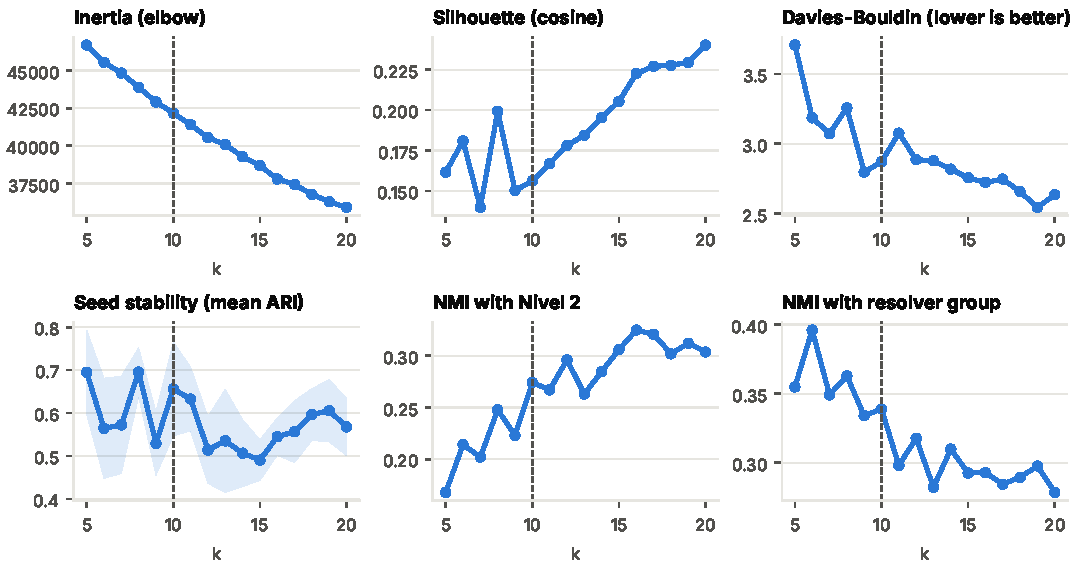
\includegraphics[width=0.9\textwidth]{cluster_sweep.pdf}
\caption{K-means sweep, $k=5\ldots20$, on LSA vectors of title + resolution note. Dashed line: selected $k=10$.
Shaded band: standard deviation of the pairwise ARI across five K-means seeds.}
\label{fig:sweep}
\end{figure*}

\subsection{Evaluation protocol}
Five stratified random splits (70/10/20\%; seeds 0--4) are created once and shared by all models. Each test set
contains 11,972 incidents. Hyperparameters are chosen on validation macro-F1 only, and each test set is scored
once. Results are reported as mean $\pm$ standard deviation over the five splits in two views:
\begin{itemize}
\item \emph{All test tickets}: operational performance, including repeated templated alerts, as in production.
\item \emph{Unseen titles}: test tickets whose cleaned title never occurs in the training split, each distinct
title counted once (about 2,270 titles per split). This measures generalization to new wording.
\end{itemize}
Metrics are accuracy, macro-F1 (each category weighted equally), weighted F1, and, for comparisons, paired
$t$-tests over splits and McNemar tests per split. Every run writes its configuration, code version, library
versions, metrics and predictions; all tables and figures are generated from these logs by script.

\subsection{Classical models}
On TF-IDF features of the title (uni- and bigrams, 50,000 features, sublinear term frequency) we train
logistic regression, linear SVM, complement naive Bayes, random forest (200 trees) and an MLP (one hidden
layer of 256 units), plus a linear SVM on word and character (3--5) n-grams to handle misspellings. Linear and
tree models use balanced class weights. Grids and selected values are listed in Appendix~\ref{app:hp}. The MLP
is trained epoch by epoch and the epoch is selected on the validation split; scikit-learn's built-in early
stopping draws a random part of the training set, which shares duplicate titles with it.

\subsection{Transformer models}
We fine-tune all layers of BETO, a Spanish BERT \cite{canete2020,devlin2019}
(\texttt{dccuchile/bert-base-spanish-wwm-cased}, 110M parameters), and XLM-RoBERTa base \cite{conneau2020}
(\texttt{FacebookAI/xlm-roberta-base}, 278M) on the anonymized title in its original form (case, accents and
word order kept, since stop-word removal discards the context these models use). The search was declared
before running: learning rate $\in\{2\cdot10^{-5}, 3\cdot10^{-5}\}$ $\times$ class-weighted loss $\in$ \{yes,
no\}, up to 8 epochs with early stopping on validation macro-F1 (patience 2), AdamW, weight decay 0.01,
10\% linear warm-up, batch size 32, maximum length 64, mixed precision on an NVIDIA T4. All eight configurations
were run on seed 0 and only validation was scored (Table~\ref{tab:search}); the best configuration of each model
was then trained on the five splits. RoBERTa-BNE was declared first but its weights are no longer available on
the Hugging Face Hub; it was replaced by XLM-RoBERTa before any result was produced.

%======================================================================
\section{Results}

\subsection{Main comparison}
\begin{table*}[!t]
\centering
\caption{Incident categorization on the held-out test set (k=10 categories, ticket title only). Mean $\pm$ standard deviation over 5 independent train/validation/test splits; about 11,972 test tickets per split. Unseen titles: test tickets whose cleaned title never occurs in training, each distinct title counted once.}
\label{tab:main}
\footnotesize
\begin{adjustbox}{max width=\textwidth}
\begin{tabular}{lcccc}
\hline
Model & Accuracy (\%) & Macro-F1 & Weighted-F1 & Macro-F1 (unseen titles) \\
\hline
BERT (BETO, tuned) & 87.2 $\pm$ 0.2 & 0.857 $\pm$ 0.003 & 0.871 $\pm$ 0.002 & 0.652 $\pm$ 0.010 \\
XLM-RoBERTa (tuned) & 87.2 $\pm$ 0.1 & 0.857 $\pm$ 0.002 & 0.871 $\pm$ 0.001 & 0.658 $\pm$ 0.011 \\
MLP (TF-IDF) & 86.8 $\pm$ 0.3 & 0.850 $\pm$ 0.005 & 0.865 $\pm$ 0.003 & 0.634 $\pm$ 0.036 \\
SVM (word+char n-grams) & 85.9 $\pm$ 0.2 & 0.847 $\pm$ 0.003 & 0.859 $\pm$ 0.002 & 0.630 $\pm$ 0.033 \\
Linear SVM & 85.9 $\pm$ 0.4 & 0.846 $\pm$ 0.005 & 0.859 $\pm$ 0.003 & 0.643 $\pm$ 0.026 \\
Random Forest & 85.2 $\pm$ 0.2 & 0.839 $\pm$ 0.003 & 0.851 $\pm$ 0.002 & 0.658 $\pm$ 0.029 \\
Complement NB & 85.1 $\pm$ 0.2 & 0.834 $\pm$ 0.002 & 0.849 $\pm$ 0.002 & 0.593 $\pm$ 0.022 \\
Logistic Regression & 83.7 $\pm$ 0.3 & 0.833 $\pm$ 0.003 & 0.841 $\pm$ 0.003 & 0.613 $\pm$ 0.028 \\
\hline
\end{tabular}
\end{adjustbox}
\end{table*}


Table~\ref{tab:main} reports all models. The two fine-tuned transformers are the best models and are tied
with each other (87.2\% accuracy, macro-F1 0.857). Paired by split on the same test tickets, both beat the
linear SVM and the word+character SVM on all five splits (macro-F1 +0.010 to +0.011, paired $t$-test
$p \le 0.017$). Against the strongest baseline, the MLP, the gain is smaller: +0.007 macro-F1, on 4/5 (BETO)
and 5/5 (XLM-RoBERTa) splits, $p=0.051$ and $p=0.034$; for accuracy the gain is +0.4 points ($p\approx0.08$).
All models stay below the 91.8\% title-only ceiling (Section~II).

The hyperparameter search mattered more than the choice of encoder: removing the class-weighted loss raised
validation macro-F1 by about two points for both models (Table~\ref{tab:search}). Our first BETO run, with
class weights and four epochs, reached 85.1\% accuracy and a macro-F1 of 0.843, below the MLP.

\begin{table}[!t]
\centering
\caption{External LLM baseline (gemini-2.5-flash, temperature 0, no thinking) against the fine-tuned and TF-IDF models on the same 1000 seed-0 test tickets (stratified sample; 200 with titles unseen in training).}
\label{tab:gemini}
\footnotesize
\begin{adjustbox}{max width=\columnwidth}
\begin{tabular}{lcccc}
\hline
Model & Acc. (\%) & Macro-F1 & Unseen acc. (\%) & Unseen macro-F1 \\
\hline
Gemini zero-shot & 73.1 & 0.733 & 68.5 & 0.589 \\
Gemini few-shot (3/class) & 74.1 & 0.739 & 66.0 & 0.570 \\
MLP (TF-IDF) & 87.8 & 0.866 & 81.5 & 0.723 \\
BETO (tuned) & 88.6 & 0.879 & 82.5 & 0.787 \\
\hline
\end{tabular}
\end{adjustbox}
\end{table}

\paragraph{External LLM baseline} As an external baseline that needs no training, Gemini~2.5~Flash classified a
stratified sample of 1,000 seed-0 test tickets from the title alone, given the category names and definitions
(zero-shot) and, in a second run, three training titles per category (few-shot). It reached 73.1\% and 74.1\%
accuracy (macro-F1 0.733 and 0.739), against 87.8\% for the MLP and 88.6\% for BETO on the same tickets, and it
also trails them on unseen titles (Table~\ref{tab:gemini}). The supervised models learn the operational
conventions of the taxonomy (templated alert titles, store codes, the boundary of the catch-all category) that
a general model cannot infer from short definitions; an LLM is therefore better used as the conversational layer
than as the classifier. Ticket-BERT~\cite{liu2023ticketbert} was not reproduced: it is trained on internal English-language Microsoft
tickets that are not available, whereas our data is in Spanish.

\subsection{Generalization to unseen titles}
On titles never seen in training, every model drops to a macro-F1 of 0.59--0.66 (last column of
Table~\ref{tab:main}). The transformers are on average 0.009--0.028 above the TF-IDF models, but the difference
is not significant ($p>0.1$). Their spread across splits is a third of the baselines' (0.010 vs.\
0.026--0.036). The gap between the two views shows that a large part of the operational accuracy comes from
recurring, templated titles, and that new wording remains the hard case.

\subsection{Errors by category}
Per-category F1 of BETO ranges from 0.58 (informational tickets) to 0.96 (Pixel Point alerts). Most errors
flow into the catch-all category 0: 24\% of informational tickets, 16\% of equipment requests and 13\% of
network incidents are predicted as category 0 (Fig.~\ref{fig:cm}). These titles often lack the detail that the
resolution note later provides.

\begin{figure*}[!t]
\centering
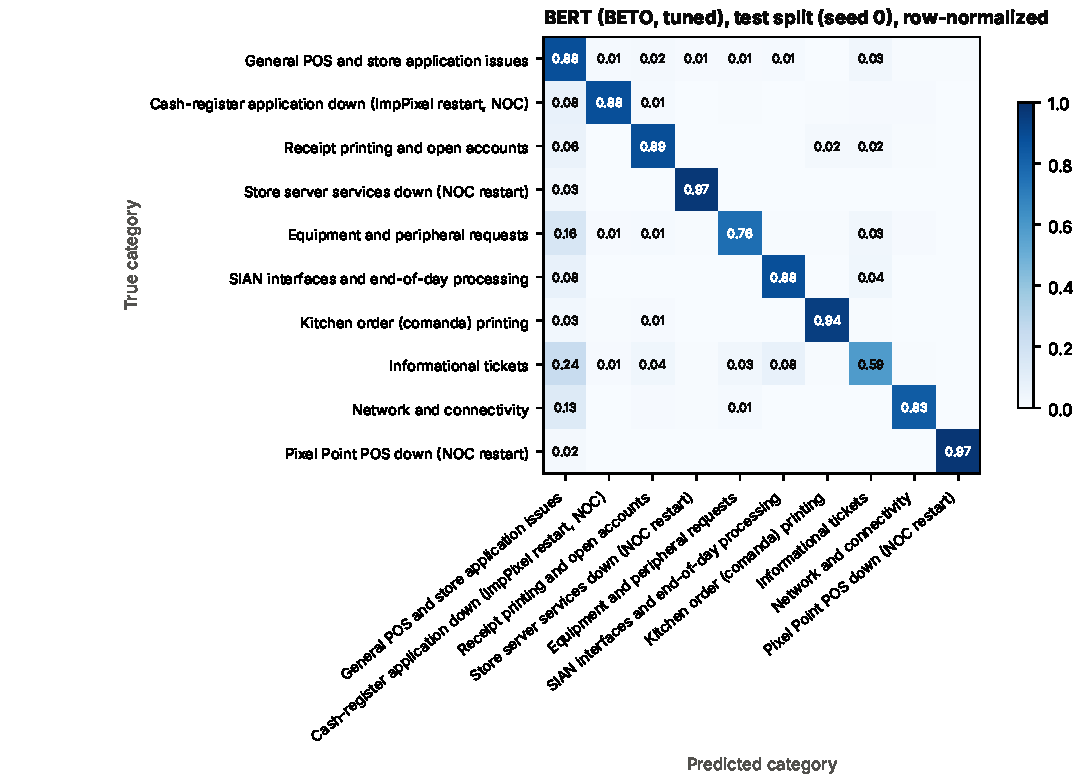
\includegraphics[width=0.78\textwidth]{confusion_best.pdf}
\caption{Row-normalized confusion matrix of fine-tuned BETO on the test split of seed 0.}
\label{fig:cm}
\end{figure*}

\subsection{Sensitivity to $k$ and to the inputs}\label{sec:ksens}
\begin{table}[!t]
\centering
\caption{Sensitivity to the number of clusters $k$: cluster quality (silhouette, seed stability as mean pairwise ARI over 5 K-means seeds, NMI with the human resolver group) and test Macro-F1 (mean $\pm$ std over 5 splits).}
\label{tab:ksens}
\footnotesize
\begin{adjustbox}{max width=\columnwidth}
\begin{tabular}{cccccc}
\hline
$k$ & Silh. & Stab. & NMI$_{grp}$ & Logistic Regression & Linear SVM \\
\hline
6 & 0.181 & 0.56 & 0.40 & 0.802 $\pm$ 0.002 & 0.824 $\pm$ 0.003 \\
8 & 0.199 & 0.70 & 0.36 & 0.803 $\pm$ 0.003 & 0.819 $\pm$ 0.004 \\
9 & 0.150 & 0.53 & 0.33 & 0.845 $\pm$ 0.002 & 0.858 $\pm$ 0.002 \\
10 & 0.156 & 0.66 & 0.34 & 0.833 $\pm$ 0.003 & 0.846 $\pm$ 0.005 \\
12 & 0.178 & 0.51 & 0.32 & 0.820 $\pm$ 0.002 & 0.831 $\pm$ 0.004 \\
15 & 0.205 & 0.49 & 0.29 & 0.841 $\pm$ 0.003 & 0.844 $\pm$ 0.003 \\
\hline
\end{tabular}
\end{adjustbox}
\end{table}

\begin{table}[!t]
\centering
\caption{Input and target ablation. The solution field is written after the ticket is resolved, so title + solution is an upper bound and not a deployable setting. The resolver-group target uses the human-assigned field Grupo Asignado instead of cluster labels.}
\label{tab:ablation}
\footnotesize
\begin{adjustbox}{max width=\columnwidth}
\begin{tabular}{llcc}
\hline
Setting & Model & Accuracy (\%) & Macro-F1 \\
\hline
Title (deployable) & Logistic Regression & 83.7 $\pm$ 0.3 & 0.833 $\pm$ 0.003 \\
Title (deployable) & Linear SVM & 85.9 $\pm$ 0.4 & 0.846 $\pm$ 0.005 \\
Title (deployable) & SVM (word+char n-grams) & 85.9 $\pm$ 0.2 & 0.847 $\pm$ 0.003 \\
Title (deployable) & Complement NB & 85.1 $\pm$ 0.2 & 0.834 $\pm$ 0.002 \\
Title + solution (upper bound) & Logistic Regression & 97.2 $\pm$ 0.1 & 0.970 $\pm$ 0.000 \\
Title + solution (upper bound) & Linear SVM & 96.9 $\pm$ 0.1 & 0.967 $\pm$ 0.001 \\
Title $\rightarrow$ resolver group & Logistic Regression & 65.2 $\pm$ 0.6 & 0.339 $\pm$ 0.021 \\
Title $\rightarrow$ resolver group & Linear SVM & 71.3 $\pm$ 0.6 & 0.381 $\pm$ 0.017 \\
Title $\rightarrow$ resolver group & Complement NB & 75.2 $\pm$ 0.3 & 0.426 $\pm$ 0.017 \\
\hline
\end{tabular}
\end{adjustbox}
\end{table}


Table~\ref{tab:ksens} repeats the linear models for $k\in\{6,8,9,10,12,15\}$. Macro-F1 varies between 0.80 and
0.86 without a trend in $k$, and $k=10$ is not the best value (it lies within the range), so the choice of $k$
was not tuned to the classifier. Table~\ref{tab:ablation} shows two controls. Adding the resolution note to the
input raises accuracy to 97\%, which confirms that the note carries the information that separates categories;
this setting is circular (the labels were derived from title + note) and not deployable. Predicting the
human-assigned resolver group from the title reaches a macro-F1 of only 0.34--0.43, which illustrates the
inconsistency of the existing labels that motivated the taxonomy.

\subsection{Confidence threshold}
\begin{table*}[!t]
\centering
\caption{Confidence threshold for the ``unclassified'' option: tickets whose top-class probability is below the threshold are left to the analyst. Coverage = share classified automatically; accuracy and macro-F1 on the classified tickets. Mean $\pm$ std over 5 splits. ECE: BERT (BETO, tuned) 0.039, XLM-RoBERTa (tuned) 0.043.}
\label{tab:confidence}
\footnotesize
\begin{adjustbox}{max width=\textwidth}
\begin{tabular}{llccc}
\hline
Model & Threshold & Coverage (\%) & Accuracy (\%) & Macro-F1 \\
\hline
BERT (BETO, tuned) & none & 100.0 $\pm$ 0.0 & 87.2 $\pm$ 0.2 & 0.857 $\pm$ 0.003 \\
BERT (BETO, tuned) & 0.50 & 98.2 $\pm$ 0.8 & 88.0 $\pm$ 0.4 & 0.865 $\pm$ 0.005 \\
BERT (BETO, tuned) & 0.60 & 94.7 $\pm$ 1.4 & 89.3 $\pm$ 0.5 & 0.877 $\pm$ 0.006 \\
BERT (BETO, tuned) & 0.70 & 90.8 $\pm$ 1.8 & 90.5 $\pm$ 0.6 & 0.889 $\pm$ 0.008 \\
BERT (BETO, tuned) & 0.80 & 85.0 $\pm$ 2.4 & 92.1 $\pm$ 0.7 & 0.905 $\pm$ 0.009 \\
BERT (BETO, tuned) & 0.90 & 76.2 $\pm$ 3.7 & 93.9 $\pm$ 0.8 & 0.924 $\pm$ 0.010 \\
BERT (BETO, tuned) & 0.95 & 64.4 $\pm$ 3.9 & 95.3 $\pm$ 0.6 & 0.940 $\pm$ 0.008 \\
XLM-RoBERTa (tuned) & none & 100.0 $\pm$ 0.0 & 87.2 $\pm$ 0.1 & 0.857 $\pm$ 0.002 \\
XLM-RoBERTa (tuned) & 0.50 & 98.3 $\pm$ 0.3 & 87.9 $\pm$ 0.1 & 0.864 $\pm$ 0.004 \\
XLM-RoBERTa (tuned) & 0.60 & 95.4 $\pm$ 0.6 & 89.1 $\pm$ 0.2 & 0.874 $\pm$ 0.003 \\
XLM-RoBERTa (tuned) & 0.70 & 91.5 $\pm$ 1.0 & 90.3 $\pm$ 0.3 & 0.886 $\pm$ 0.004 \\
XLM-RoBERTa (tuned) & 0.80 & 86.2 $\pm$ 1.2 & 91.8 $\pm$ 0.3 & 0.900 $\pm$ 0.005 \\
XLM-RoBERTa (tuned) & 0.90 & 76.8 $\pm$ 1.4 & 93.8 $\pm$ 0.2 & 0.922 $\pm$ 0.005 \\
XLM-RoBERTa (tuned) & 0.95 & 65.7 $\pm$ 3.9 & 95.3 $\pm$ 0.4 & 0.942 $\pm$ 0.008 \\
\hline
\end{tabular}
\end{adjustbox}
\end{table*}


The deployed classifier can leave a ticket ``unclassified'' when its top probability is below a threshold
(Table~\ref{tab:confidence}, Fig.~\ref{fig:conf}). For BETO, a threshold of 0.8 classifies $85.0\pm2.4$\% of
tickets automatically with $92.1\pm0.7$\% accuracy; 0.9 classifies 76.2\% with 93.9\%. The expected
calibration error is 0.039 (BETO) and 0.043 (XLM-RoBERTa), so probabilities can be used as confidence without
recalibration.

\begin{figure}[!t]
\centering
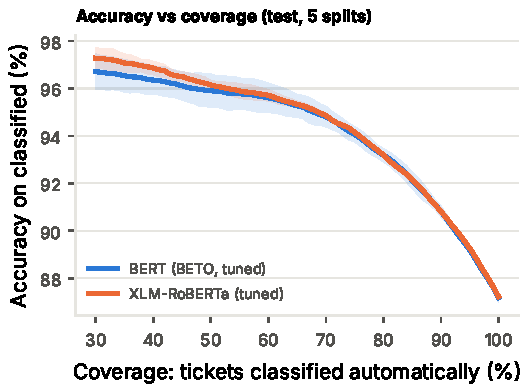
\includegraphics[width=\columnwidth]{confidence_coverage.pdf}
\caption{Accuracy on automatically classified tickets versus coverage, mean (line) and standard deviation
(band) over five splits.}
\label{fig:conf}
\end{figure}

\subsection{Cost}
\begin{table}[!t]
\centering
\caption{Inference cost of a single new ticket on CPU (raw title $\rightarrow$ cleaning $\rightarrow$ TF-IDF $\rightarrow$ prediction), 1,000 test tickets, one process.}
\label{tab:latency}
\footnotesize
\begin{adjustbox}{max width=\columnwidth}
\begin{tabular}{lccc}
\hline
Model & Median (ms) & p95 (ms) & Size (MB) \\
\hline
Logistic Regression & 0.62 & 0.89 & 0.8 \\
Linear SVM & 0.49 & 0.81 & 0.8 \\
SVM (word+char n-grams) & 0.99 & 1.14 & 1.8 \\
Complement NB & 0.54 & 0.60 & 1.3 \\
Random Forest & 44.62 & 56.05 & 307.5 \\
MLP (TF-IDF) & 0.62 & 1.10 & 51.7 \\
\hline
\end{tabular}
\end{adjustbox}
\end{table}


TF-IDF models classify a ticket on CPU in under 1 ms (median, full path from raw title to prediction) with
models of 1--2 MB, except random forest (45 ms, 308 MB) (Table~\ref{tab:latency}). BETO needs 0.7 ms per ticket
in batches on a T4 GPU and occupies 440 MB; XLM-RoBERTa occupies 1.1 GB and took 28 minutes per training run
versus 15 for BETO. Because the two transformers are tied, BETO is preferred when a GPU is available; the
deployed service uses the MLP (Section~\ref{sec:architecture}).

%======================================================================
\section{Solution Architecture}\label{sec:architecture}

Fig.~\ref{fig:arch} shows the architecture. It has two parts.

\paragraph{Classifier service} The classifier is published as a private API on Google Cloud Run. Given the
user's description it returns the category, its probability and the top-3 categories, and ``unclassified'' when
the probability is below the 0.8 threshold (Table~\ref{tab:confidence}). The deployed model is the MLP on word
TF-IDF features (seed-0 training split; 86.7\% test accuracy), not BETO: it is within 0.4 points of the best
transformer (Table~\ref{tab:main}), needs no GPU, and classifies a single ticket in about 1~ms on one CPU
(Table~\ref{tab:latency}); BETO remains the best model offline. At the 0.8 threshold the deployed MLP
classifies 80.7\% of the seed-0 test tickets automatically with 92.2\% accuracy (ECE 0.020), close to BETO's
85.0\% and 92.1\% (Table~\ref{tab:confidence}). The same service retrieves similar resolved incidents. The
user's free text is cleaned with the same normalization as the training titles; no name lists are shipped.
From the agent, a call to the service takes 39~ms (median round trip on Cloud Run, warm instance); a cold start
of the service adds about 9~s.

\paragraph{First-contact agent} An agent built on Vertex AI with Gemini~2.5~Flash is the first point of contact
for store staff in Microsoft Teams. When a user reports a problem, the agent asks at most two short questions
(affected system and store, since when, what was already tried) or declines requests that are not IT incidents.
It then calls the classifier and retrieves the five most similar resolved incidents, filtered by the predicted
category only when its probability is at least 0.8 (Section~\ref{sec:retrieval}). Gemini proposes up to four
steps that the user can safely perform, using only actions present in the retrieved cases; steps that need
remote access or a technician are not proposed to the user. The agent then asks whether the problem was solved.
If it was, a ticket is created and closed as resolved at first contact; if it was not, or if no safe steps
exist, a ticket is created for the technician with the summary, the conversation, the classifier's category and
probability, and the retrieved cases, so the technician starts from a categorized ticket with candidate
solutions instead of a blank form. Tickets are created in Jira Service Management through its REST API; the
ticketing back end is an interchangeable tool, and another ticketing platform can be connected
through the same interface. The agent does not replace the technician. The knowledge base contains the
12,848 training-split incidents whose resolution note has at least four informative words, deduplicated and
anonymized with the same rules as the shared dataset; test tickets are excluded to avoid leakage. Each
conversation is logged (category, probability, filter, retrieved cases, decision, time to first proposal) for
the evaluation below.

\begin{figure}[!t]
\centering
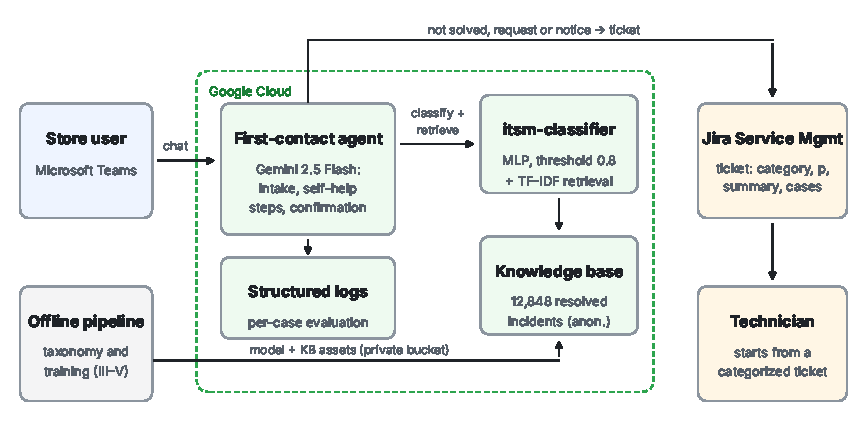
\includegraphics[width=\columnwidth]{architecture.pdf}
\caption{Deployed architecture: the first-contact agent (Vertex AI, Gemini) in Microsoft Teams calls the private
classifier and retrieval service on Cloud Run, whose model and knowledge base are produced offline (Sections
III--V); tickets are created in Jira Service Management, and every case is logged for evaluation.}
\label{fig:arch}
\end{figure}

\subsection{Retrieval evaluation}\label{sec:retrieval}
\begin{table*}[!t]
\centering
\caption{Offline evaluation of the retrieval step (top-5 similar resolved incidents from the training split; TF-IDF retriever as a proxy for the agent's search). Hit: a retrieved case has the query's true category. Resolution similarity: max cosine between the query's actual resolution note and the retrieved notes. Mean $\pm$ std over 5 splits; about 7,821 queries (all) and 1,304 (unseen titles) per split.}
\label{tab:retrieval}
\footnotesize
\begin{adjustbox}{max width=\textwidth}
\begin{tabular}{lcccc}
\hline
Retrieval filter & Hit@5 (all) & Res. sim. (all) & Hit@5 (unseen) & Res. sim. (unseen) \\
\hline
No filter & 0.845 $\pm$ 0.072 & 0.309 $\pm$ 0.082 & 0.821 $\pm$ 0.004 & 0.221 $\pm$ 0.005 \\
Predicted category (always) & 0.840 $\pm$ 0.003 & 0.386 $\pm$ 0.062 & 0.702 $\pm$ 0.011 & 0.200 $\pm$ 0.008 \\
Predicted category if $p\ge0.8$ & 0.879 $\pm$ 0.007 & 0.391 $\pm$ 0.063 & 0.772 $\pm$ 0.020 & 0.211 $\pm$ 0.006 \\
True category (oracle) & 1.000 $\pm$ 0.000 & 0.441 $\pm$ 0.061 & 1.000 $\pm$ 0.000 & 0.308 $\pm$ 0.005 \\
\hline
\end{tabular}
\end{adjustbox}
\end{table*}


The retrieval step is evaluated offline on every test incident with a recorded resolution note, against a
knowledge base of about 16,000 training incidents (Table~\ref{tab:retrieval}). A TF-IDF retriever on the title
serves as a transparent proxy for the agent's search. Two results guide the design. First, the category is
useful: restricting retrieval to the true category raises the similarity between retrieved and actual
resolutions from 0.31 to 0.44 (all tickets) and from 0.22 to 0.31 (unseen titles). Second, the predicted category
is only useful when it is reliable: always filtering by it lowers the share of queries with a same-category case
among the top five on unseen titles (0.82 to 0.70), because a misclassified ticket is cut off from the right
cases. Filtering only when the classifier's probability is at least 0.8 gives the best result on all tickets
(hit 0.88, similarity 0.39) and limits the loss on unseen titles; the agent therefore applies the category filter
only above the confidence threshold. On all tickets, results without a filter vary strongly across splits because
hundreds of templated alerts share the same title and the retrieved cases among them differ.

\subsection{Agent evaluation on held-out cases}
\begin{table}[!t]
\centering
\caption{Automated evaluation of the deployed agent on 30 held-out test incidents and 5 out-of-scope requests (simulated store user: gemini-2.5-flash; judge: gemini-3.1-pro-preview). Out-of-scope requests correctly declined: 5/5, tickets created for them: 0.}
\label{tab:agent_eval_v2}
\footnotesize
\begin{adjustbox}{max width=\columnwidth}
\begin{tabular}{lccc}
\hline
Metric & All in-scope & Seen wording & Unseen wording \\
\hline
Cases (n) & 30 & 10 & 20 \\
Classifier category correct & 50\% & 50\% & 50\% \\
Classifier confident ($p\ge0.8$) & 57\% & 80\% & 45\% \\
Agent proposed steps & 57\% & 70\% & 50\% \\
Steps would solve (of proposals) & 24\% & 29\% & 20\% \\
Resolved at first contact (of all) & 13\% & 20\% & 10\% \\
Steps grounded in retrieved cases & 71\% & 57\% & 80\% \\
Hallucinated steps (of proposals) & 29\% & 43\% & 20\% \\
Ticket created when not solved & 96\% & 88\% & 100\% \\
Wrongly declined as not IT (n) & 1 & 1 & 0 \\
Registered as request/notice (n) & 6 & 0 & 6 \\
Questions asked (mean) & 0.8 & 0.9 & 0.7 \\
\hline
\end{tabular}
\end{adjustbox}
\end{table}


A reduced, automated evaluation runs the deployed agent, through the same code path that serves Teams, on 35
cases fixed before the agent was built: 30 held-out test incidents (three per category, 20 of them with wording
not seen in training) and five out-of-scope requests (e.g., an air-conditioning failure or a payroll question).
A simulated store user (Gemini~2.5~Flash) turns each ticket title into a chat report and answers the agent's
questions without knowing the resolution. A judge from a different, larger model (Gemini~3.1~Pro) compares the
proposed steps with the actual resolution and with the retrieved cases and scores whether they would solve the
problem, whether each step is grounded in a retrieved case, and whether any step or system is invented; the
simulated user confirms the problem as solved only if the judge says the steps would solve it. Category, decision,
ticket and timing are recorded automatically. Table~\ref{tab:agent_eval_v2} reports the results. To check the
judge, the author rated eight of the proposals blind to its verdict: he considered all eight would solve the
problem and none invented, whereas the judge accepted two and flagged three as containing unsupported steps
(agreement 25\% and 62.5\%). The judge is therefore much stricter than a domain expert, and the first-contact
resolution and hallucination figures below should be read as a conservative bound.

The agent declined all five out-of-scope requests without creating tickets and created a ticket in 25 of the 26
in-scope cases that it did not resolve. Four results temper the picture. First, the classifier assigns the correct
category to only 50\% of the conversational reports, against 87\% on ticket titles: users describe symptoms in
words that differ from technicians' titles, and the three categories of automatic monitoring alerts (cash-register
application, store server and Pixel Point down) are rarely reported by users at all, so their reports fall into the
general POS category. Above the threshold (57\% of cases) the category is right only 53\% of the time, so the
threshold calibrated on titles does not transfer to chat text. Second, only 13\% of the cases are resolved at first
contact: most actual resolutions require a technician with remote access (restarting server services,
reconfiguring a printer queue), which the agent correctly does not ask the user to do. Third, 29\% of the proposals
contain at least one step not supported by the retrieved cases (typically generic advice such as checking cables);
none was unsafe, but this is the main failure mode to address. Fourth, a first run (agent v1) declined four
in-scope cases (two informational notices and two software-installation requests) as not IT; the intake prompt was
then changed to register IT requests and notices directly, and the run reported here (v2) declined one. Because
this change was made after seeing the v1 results on the same cases, the v2 figures are optimistic for that
behavior; the v1 run is reported in the repository. The median time from the first message to the proposal was
18~s, and the classifier service answered in 39~ms (median round trip from the agent).

\begin{figure}[!t]
\centering
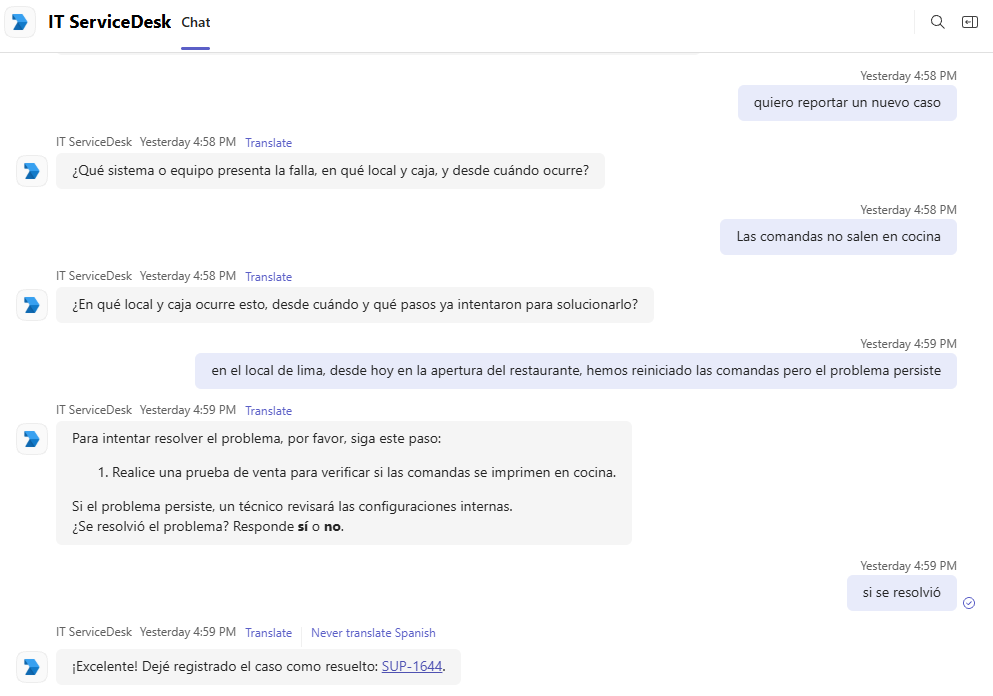
\includegraphics[width=\columnwidth]{teams_agent.png}
\caption{The deployed first-contact agent in Microsoft Teams (illustration, not evidence of performance): it asks
for the missing details, proposes a step taken from similar resolved incidents, asks whether the problem was solved
and records the case in Jira (ticket created and closed as resolved at first contact).}
\label{fig:teams}
\end{figure}

%======================================================================
\section{Discussion and Limitations}

\paragraph{Pseudo-labels} The categories are cluster assignments, and the sweep shows weak cluster structure.
Accuracy measures agreement with this taxonomy, not with an independent human truth; the label audit estimates
how far an expert would confirm the taxonomy: an LLM rater confirmed 88.7\% of the labels, but the author agreed
with only 57.6\% of them on a blind subsample (74.6\% after merging the three alert categories). Part of the
disagreement comes from ambiguous names of the alert categories, part from the heterogeneous catch-all and
informational categories, and part from tickets mis-recorded as incidents in the source system. All accuracies
in this paper therefore measure agreement with the cluster taxonomy, and could be considerably lower against
expert labels. The human check covers 59 tickets from a single rater, who also approved the names; a larger audit
with several independent analysts, and clearer names for the alert categories, are needed.

\paragraph{Ceiling and templated alerts} Title-only accuracy is bounded at 91.8\%, and templated alerts make some
categories easy. Accuracy alone overstates generalization; the unseen-title view (macro-F1 $\approx$ 0.65) is the
more conservative estimate.

\paragraph{Out-of-distribution incidents} New systems, stores or failure modes after October 2024 are not
represented. The confidence threshold routes uncertain tickets to a human, and the taxonomy must be reviewed
periodically.

\paragraph{Cost and latency} The transformer adds a GPU or a larger CPU instance and hundreds of megabytes of
memory for a gain of 0.4--1.3 accuracy points over TF-IDF models that run in under a millisecond; for
organizations without that capacity, the word+character SVM is a reasonable alternative.

\paragraph{Hallucination and hand-off} Generated proposals can be wrong or unsupported, and a user may follow
them without a technician. Retrieval is restricted to resolved incidents, the agent creates a ticket whenever the
problem is not confirmed as solved; in the 35-case evaluation 29\% of the proposals contained unsupported steps,
so grounding must be enforced more strictly (e.g., by quoting the retrieved action) before deployment at scale. A larger evaluation with several raters is needed before claiming effects on FCR.

\paragraph{Agent evaluation scope} The agent evaluation is reduced: an offline proxy for retrieval and 35 cases
with a simulated user and an LLM judge. Both the user and the judge are language models; the judge was not
validated against human ratings beyond an eight-case check, in which it was much stricter than the author, and a
simulated user may describe problems more clearly or more uniformly than store staff. With 30 in-scope cases, each percentage has a wide confidence interval (about $\pm$15--18 points).
The evaluation shows feasibility and failure modes, not production impact; a study with real users and several
human raters is needed before claiming effects on first-contact resolution.

\paragraph{Scope} The data come from one organization, one language variety and ten months. Results may not
transfer to other sectors without re-deriving the taxonomy.

%======================================================================
\section{Conclusion and Future Work}

This work built and evaluated an end-to-end pipeline for incident categorization and a user-facing first-contact agent on
59,860 real Spanish-language incidents. A static ten-category taxonomy was derived by clustering titles and
resolution notes and named for use in reporting and in the interface. Under a reproducible protocol, fine-tuned
BETO and XLM-RoBERTa were the best title-only classifiers (87.2\% accuracy, macro-F1 0.857), with a small but
consistent margin over TF-IDF baselines, below a ceiling of 91.8\% imposed by the labels. On unseen wording all
models drop to a macro-F1 of about 0.65. A confidence threshold of 0.8 lets the classifier label 85\% of tickets
at 92\% accuracy and leave the rest to a technician. The classifier is the entry point of a user-facing Vertex AI
agent; offline, filtering retrieval by the predicted category helps only when the classifier is confident, so the
agent applies the filter above the threshold. In a reduced automated evaluation the deployed agent declined all
out-of-scope requests and escalated unresolved cases, but it resolved only 13\% of the incidents at first contact
(most require a technician), the classifier was right on 50\% of conversational reports, and 29\% of proposals
contained unsupported steps. A blind check by the service desk lead confirmed 57.6\% of the cluster labels (74.6\%
after merging the three alert categories), so the reported accuracies measure agreement with the cluster
taxonomy rather than with expert labels.

Future work: (1) a full agent evaluation with real users and several raters and its effect on MTTR and FCR in
production, together with training the classifier on conversational reports and enforcing stricter grounding; (2) map
categories to resolver groups for automatic routing; (3) continue pre-training BETO on ticket text
(domain-adaptive pre-training); (4) hierarchical categories for the catch-all class; (5) periodic
re-derivation of the taxonomy to handle drift; and (6) replicating the pipeline (clustering, naming, supervised
training) on a public helpdesk dataset to test how far the findings generalize beyond one organization.

\section*{Data and Code Availability}
The anonymized dataset (59,860 incidents: pseudonymous id, anonymized title, category, resolver group and the
five splits), its data card, and all code, configuration files and run logs are available at
\url{https://github.com/crobregon-itexpert/itsm-incident-categorization} (code under MIT, data under CC BY 4.0).
All tables and figures in this paper are generated from the logs by \texttt{python -m itsm.report}. The
components of the deployed agent are included; its model and knowledge-base assets, built from private data, are
not.

\section*{Author Contributions}
C.~Obregón: conceptualization, data curation, methodology, software, validation, investigation, writing---original
draft, review and editing. \pending{Confirm the list of authors and roles.}

\section*{Funding}
This research received no external funding; its costs, including cloud services, were covered by the author.

\section*{Institutional Review Board Statement}
Not applicable: the study uses historical service-desk records and no experiment with human participants; the
agent evaluation uses a simulated user.

\section*{Data Statement}
The incidents are real operational records of the service desk. They were anonymized before analysis and
release: the organization is not identified, and personal names, store identifiers and digits are masked in
titles and resolution notes, with words that occur in fewer than five tickets replaced by a placeholder. In the
public file, company, group and brand identifiers are additionally replaced by neutral codes through a one-to-one
word substitution applied after the experiments, which leaves word-level features unchanged. Only
the fields needed to reproduce the experiments are released.

\section*{Conflicts of Interest}
The author declares no conflict of interest.

\section*{Use of Generative AI}
Large language models are components of the system and of its evaluation: Gemini~2.5~Flash runs the agent and the
simulated user, Gemini~3.1~Pro is the evaluation judge, and Gemini~2.5~Flash is the external classification baseline
and the second rater of the label audit, as described in the text. During the preparation of this work, the author
used Claude (Anthropic) to write and review analysis and deployment code, to run and log the experiments, and to
draft and edit the manuscript and the response to reviewers. The author reviewed all content and takes full
responsibility for the accuracy and integrity of the published article.

\appendices
\section{Hyperparameters}\label{app:hp}
Classical models (scikit-learn \cite{pedregosa2011}), selected on validation macro-F1: logistic regression
$C\in\{0.25,1,4,16\}$; linear SVM $C\in\{0.03,0.1,0.5,1\}$; word+character SVM $C\in\{0.1,0.5,1\}$, character
n-grams 3--5 (\texttt{char\_wb}, 100,000 features); complement naive Bayes $\alpha\in\{0.03,0.1,0.3,1\}$;
random forest 200 trees, balanced subsample weights; MLP 256 hidden units, Adam, learning rate $10^{-3}$, batch
256, $L_2$ $\alpha\in\{10^{-4},10^{-2}\}$, up to 20 epochs, patience 3 on validation. The selected value for
every split is stored in the run logs. Transformer settings are in Table~\ref{tab:search}.

\begin{table}[!t]
\centering
\caption{Transformer hyperparameter search (declared before running): validation macro-F1 on seed 0; the test split was not scored for any configuration in this stage. Fixed: AdamW, weight decay 0.01, linear warm-up 10\%, batch 32, max length 64, up to 8 epochs, early stopping patience 2, mixed precision, full fine-tuning, NVIDIA T4.}
\label{tab:search}
\footnotesize
\begin{adjustbox}{max width=\columnwidth}
\begin{tabular}{lccccc}
\hline
Model & LR & Class weights & Val. Macro-F1 & Best epoch & Min \\
\hline
XLM-RoBERTa base (selected) & 2e-05 & no & 0.866 & 6 & 30 \\
BETO & 2e-05 & no & 0.865 & 3 & 11 \\
XLM-RoBERTa base & 3e-05 & no & 0.864 & 2 & 15 \\
BETO & 3e-05 & no & 0.863 & 3 & 12 \\
XLM-RoBERTa base & 3e-05 & yes & 0.855 & 4 & 23 \\
XLM-RoBERTa base & 2e-05 & yes & 0.847 & 4 & 23 \\
BETO & 2e-05 & yes & 0.847 & 4 & 14 \\
BETO & 3e-05 & yes & 0.842 & 2 & 9 \\
\hline
\end{tabular}
\end{adjustbox}
\end{table}

\begin{table}[!t]
\centering
\caption{K-means on LSA vectors of title + solution: internal quality, stability and agreement with human fields for $k=5\ldots20$.}
\label{tab:sweep}
\footnotesize
\begin{adjustbox}{max width=\columnwidth}
\begin{tabular}{ccccccc}
\hline
$k$ & Silh. & DB & Stab. & Largest (\%) & NMI$_{N2}$ & NMI$_{grp}$ \\
\hline
5 & 0.162 & 3.71 & 0.70 & 42.2 & 0.17 & 0.35 \\
6 & 0.181 & 3.19 & 0.56 & 46.9 & 0.21 & 0.40 \\
7 & 0.140 & 3.07 & 0.57 & 44.2 & 0.20 & 0.35 \\
8 & 0.199 & 3.26 & 0.70 & 34.4 & 0.25 & 0.36 \\
9 & 0.150 & 2.80 & 0.53 & 42.9 & 0.22 & 0.33 \\
10 & 0.156 & 2.87 & 0.66 & 37.9 & 0.27 & 0.34 \\
11 & 0.167 & 3.08 & 0.63 & 27.9 & 0.27 & 0.30 \\
12 & 0.178 & 2.89 & 0.51 & 30.4 & 0.30 & 0.32 \\
13 & 0.184 & 2.88 & 0.54 & 26.6 & 0.26 & 0.28 \\
14 & 0.195 & 2.82 & 0.51 & 23.5 & 0.28 & 0.31 \\
15 & 0.205 & 2.76 & 0.49 & 20.2 & 0.31 & 0.29 \\
16 & 0.223 & 2.72 & 0.54 & 16.8 & 0.32 & 0.29 \\
17 & 0.227 & 2.75 & 0.56 & 19.4 & 0.32 & 0.28 \\
18 & 0.228 & 2.66 & 0.60 & 18.9 & 0.30 & 0.29 \\
19 & 0.230 & 2.54 & 0.61 & 20.9 & 0.31 & 0.30 \\
20 & 0.240 & 2.63 & 0.57 & 17.1 & 0.30 & 0.28 \\
\hline
\end{tabular}
\end{adjustbox}
\end{table}


\begin{thebibliography}{00}
\bibitem{itil4} AXELOS, \emph{ITIL\textsuperscript{\textregistered} 4 Foundation}. London, U.K.: AXELOS Ltd., 2019.
\bibitem{zangari2023} A. Zangari, M. Marcuzzo, M. Schiavinato, A. Gasparetto, and A. Albarelli, ``Ticket
automation: An insight into current research with applications to multi-level classification scenarios,''
\emph{Expert Syst. Appl.}, vol. 225, Art. no. 119984, 2023.
\bibitem{zendesk} Zendesk, ``What is first contact resolution (FCR)? Benefits + best practices,'' Zendesk Blog,
2024. [Online]. Available: https://www.zendesk.com/blog/first-contact-resolution-friend-foe-frenemy/
\bibitem{sarwar2023} M. I. Sarwar, Q. Abbas, T. Alyas, A. Alzahrani, T. Alghamdi, and Y. Alsaawy, ``Digital
transformation of public sector governance with IT service management---A pilot study,'' \emph{IEEE Access},
vol. 11, pp. 6490--6512, 2023, doi: 10.1109/ACCESS.2023.3237550.
\bibitem{ignaim2024} K. M. Ignaim and J. M. Fernandes, ``Improving incident management processes with feature
models,'' \emph{J. Cyber Secur. Mobil.}, vol. 13, no. 4, pp. 701--724, 2024, doi: 10.13052/jcsm2245-1439.1346.
\bibitem{revina2020} A. Revina, K. Buza, and V. G. Meister, ``IT ticket classification: The simpler, the
better,'' \emph{IEEE Access}, vol. 8, pp. 193380--193395, 2020, doi: 10.1109/ACCESS.2020.3032840.
\bibitem{ramya2018} C. Ramya, S. P. Paramesh, and K. S. Shreedhara, ``Classifying the unstructured IT service
desk tickets using ensemble of classifiers,'' in \emph{Proc. 3rd Int. Conf. Comput. Syst. Inf. Technol.
Sustainable Solutions (CSITSS)}, 2018; arXiv:2103.15822.
\bibitem{liu2023ticketbert} Z. Liu, C. Benge, and S. Jiang, ``Ticket-BERT: Labeling incident management
tickets with language models,'' 2023, arXiv:2307.00108.
\bibitem{ahmed2022} S. Ahmed, M. Singh, B. Doherty, E. I. Ramlan, K. Harkin, and D. Coyle, ``Multiple
severity-level classifications for IT incident risk prediction,'' in \emph{Proc. 9th Int. Conf. Soft Comput.
Mach. Intell. (ISCMI)}, 2022, pp. 270--274, doi: 10.1109/ISCMI56532.2022.10068477.
\bibitem{le2025} M. T. Lê and A. Ait Bachir, ``Learning to prioritize IT tickets: A comparative evaluation of
embedding-based approaches and fine-tuned transformer models,'' 2025, arXiv:2512.17916.
\bibitem{razma2026} A. Razma and R. Jurkus, ``AI-based classification of IT support requests in enterprise
service management systems,'' \emph{Systems}, vol. 14, no. 2, Art. no. 223, 2026, doi: 10.3390/systems14020223.
\bibitem{song2023} H. Song, M. Kim, D. Park, Y. Shin, and J.-G. Lee, ``Learning from noisy labels with deep
neural networks: A survey,'' \emph{IEEE Trans. Neural Netw. Learn. Syst.}, vol. 34, no. 11, pp. 8135--8153, 2023.
\bibitem{lewis2020} P. Lewis et al., ``Retrieval-augmented generation for knowledge-intensive NLP tasks,'' in
\emph{Adv. Neural Inf. Process. Syst. (NeurIPS)}, vol. 33, 2020, pp. 9459--9474.
\bibitem{isaza2024} P. T. Isaza et al., ``Retrieval augmented generation-based incident resolution
recommendation system for IT support,'' 2024, arXiv:2409.13707.
\bibitem{devlin2019} J. Devlin, M.-W. Chang, K. Lee, and K. Toutanova, ``BERT: Pre-training of deep
bidirectional transformers for language understanding,'' in \emph{Proc. NAACL-HLT}, 2019, pp. 4171--4186.
\bibitem{canete2020} J. Cañete, G. Chaperon, R. Fuentes, J.-H. Ho, H. Kang, and J. Pérez, ``Spanish pre-trained
BERT model and evaluation data,'' in \emph{Proc. PML4DC Workshop, ICLR}, 2020.
\bibitem{conneau2020} A. Conneau et al., ``Unsupervised cross-lingual representation learning at scale,'' in
\emph{Proc. 58th Annu. Meeting Assoc. Comput. Linguist. (ACL)}, 2020, pp. 8440--8451.
\bibitem{pedregosa2011} F. Pedregosa et al., ``Scikit-learn: Machine learning in Python,'' \emph{J. Mach. Learn.
Res.}, vol. 12, pp. 2825--2830, 2011.
\end{thebibliography}

\end{document}
